\section{Event storage}
\large \textbf{Apache Kafka}\\
\normalsize
\textbf{Durable storage}

In Kafka, records are stored in partitions each of which is stored on the disk as a number of segment files \cite{kafkalog}. The broker receives records and writes them sequentially to these files. When a segment file reaches its configurable maximum size, a new file will be created for writing new records. Since all records are only appended to these files, the read/write of records only requires sequential I/O on the disk. This is one of the key design features of Kafka to help maintain fast performance even on cheap hard disks.  

However, a Kafka broker can already acknowledge writing requests when records are written to I/O buffer and not necessarily when records are persisted to disk. Therefore, durability is not guaranteed, and message loss can still happen when the broker fails before flushing records to disk. User can force disk flush to ensure durability whenever a message is received but this is not recommended by Kafka since it can reduce the throughput of the system \cite{kafkaflushmessage}. To achieve durability, a more common approach is combining this unflushed write feature with redundant write on other brokers in the cluster which is the fault-tolerance feature for storage provided by Kafka. This is elaborated in more detail in the next section.

\textbf{Event storage is fault tolerant}\\
As briefly mentioned in the general concept, there are two types of Kafka partitions, namely, leader and follower. The leader partition is active and can serve read/write requests from clients while followers are standby replicas of the leader. For fault tolerance, Kafka supports data replication among brokers in the cluster \cite{kafkadatareplication}. For each topic, user can specify a replication factor which determines the number of existing copies of records on Kafka.  When replication factor is 2 or more, every partition of the topic will have 1 leader and 1 or more followers. For each partition, each of its copies will be distributed on a different broker in the cluster. Therefore, there will be no single point of failure for record storage. The replication factor must be equal or smaller than the number of brokers in the Kafka cluster.

However, enabling only data replication on the broker cannot guarantee that all records are safely replicated on the Kafka cluster.  By default, a Kafka producer sends a record and only waits for the acknowledgement of successful write from the leader partition. If the broker with the leader partition goes down before the record is flushed to its disk and replicated to other follower replications, the record may be lost without the producer knowing about it for resending. Therefore, the producer must be strictly configured to wait for acknowledgements from the leader partition as well as other follower replicas. In this case, the leader partition will also wait for acknowledgements from its followers before confirming with client. By having the redundant acknowledgements, durability is guaranteed even when messages are not yet persisted to disks given that all brokers retain the partition do not fail simultaneously. 
\begin{figure}[h]
	\centering
	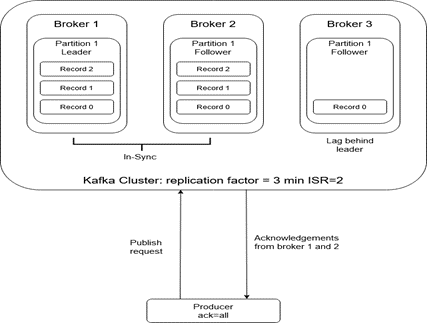
\includegraphics[width=8cm,height=6.5cm]{images/ft-eventstorage-kafka.png}
	\caption{Data replication model for fault tolerance of event storage on Kafka.}
	\label{fig:fteventstorekafka}
\end{figure}

For each replicated partition, the follower periodically fetch data from leader to stay in-sync. If the producer waits for acknowledgements from all replicas, some followers may fall too far behind the leader for instance due to network connection and increase the waiting time of the producer. Therefore, the leader of the partition dynamically maintains a list of in-sync replicas (ISR) which contains itself and all followers which currently stays synchronized with it. This list is stored on Zookeeper. When a follower does not catch up with the leader by sending fetch request after a configured amount of time, it will be removed from the ISR of the partition. The slow follower can rejoin ISR later when it has fully caught up with the leader partition. In practice, the producer will only wait for acknowledgements from the ISR instead of all replicas. This aims at balancing between the durability, fault-tolerance of published records and the latency for acknowledgment. As a result, a message acknowledged to producer can survive up to \emph{ISR-1} failed nodes and still be available to consumer.

It could be possible that all followers of a partition are out-of-sync with the leader. In this case, producer only receives one acknowledgment from the leader which brings back the problem of losing messages. Therefore, Kafka also provides the option to configure the minimum number of in-sync replicas. If the ISR falls below this number, new writing requests will be rejected, and availability is compromised to ensure the durability.

Durability and fault tolerance of data storage on Kafka are closely related to each other and can only be achieved with the right configurations on both Kafka brokers and Kafka producers. In addition, Kafka provides many configuration options to give users the flexibility to choose different priorities for their systems such as availability, durability, latency. 

\textbf{Flexible data retention policy}\\
All records published to Kafka will be retained. Old data can be cleaned up with different cleanup policies \cite{kafkacleanuppolicy}. These policies can be configured on the broker level which will then be applied to all topics or they can be configured differently for individual topic. There are two basic strategies to retain data:
\begin{itemize}
	\item Delete: All records are retained for a period of time or based on a maximum size and then they will be deleted.
	\item Compact: This strategy is only applicable to records with key values. The topic will be compacted. Only the latest record of each key value is retained.
\end{itemize}

For the first strategy, user can choose different retention policies for a partition based on maximum size or for a segment file of a partition based on retention period. Once the retention limit is exceeded, oldest segment file of the partition will be deleted. By default, there is no limit on the size of a partition and the retention period is 7 days. User can also configure infinite retention period if necessary.

\begin{figure}[h]
	\centering
	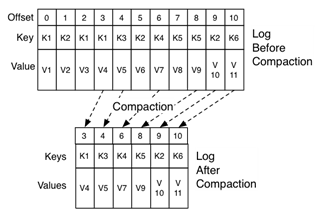
\includegraphics[width=6.5cm,height=5.5cm]{images/compact-kafka.png}
	\caption{Log compaction on Kafka (taken from Kafka documentation \cite{kafkadocumentation}).}
	\label{fig:compactekafka}
\end{figure}
For the second strategy, the background cleaner thread of Kafka will regularly scan the segment files and keep only the latest record for each key value (Figure \ref{fig:compactekafka}). Therefore, this only works with records with non-empty key value. Writing request of record without a key to a topic configured with compact cleanup policy will be rejected.


The two strategies can also be combined. With this setup, topics will be compacted regularly but when the retention maximum size or maximum retention period is reached, the data will also be removed regardless of being compacted or not. For example, in case of an online shopping application where each order is kept track by a sequence of events published to Kafka as records, when users are interested in the latest status of an order but only if the order is not older than 3 months, it is reasonable to this combination of retention strategies.

To sum up, Kafka provides a flexible way to retain all records or only selective data. Users can choose the appropriate strategy based on their use cases. 

\large \textbf{Apache Pulsar}\\
\normalsize
\textbf{Durable storage}

A Pulsar topic can be persistent or non-persistent which must be specified by user when creating the topic. Messages on non-persistent topics are only kept in-memory on the Pulsar brokers. For persistent topics, Pulsar provides the persistence layer using Bookkeeper.  A Pulsar broker has a Bookkeeper client internally. When receiving writing requests from clients, Pulsar broker sends persistent requests to the Bookkeeper cluster. Bookkeeper provides the storage abstraction called ledger. A Pulsar topic is made up from one or more ledgers. New messages will be appended to the end of a ledger. Once a ledger reaches its maximum size or the Bookkeeper node (Bookie) is restarted, a new ledger will be created. Internally, a Bookie store messages of a ledger in an entry log file on its disk. Durability of data on a Bookie is guaranteed once an acknowledgement is sent back to Pulsar broker. The broker then can confirm the successful write with client.

\textbf{Event storage is fault tolerant}\\
Pulsar supports replication of messages of a topic on multiple Bookies for fault-tolerance. To achieve this, Pulsar utilizes the built-in replication mechanism of Bookkeeper. A Pulsar topic comprises of one or more Bookkeeper ledgers. Each ledger can be further made from one or more fragments. When a ledger is created, it must have three important configuration options which control how messages on the ledger are written and replicated on Bookkeeper cluster \cite{bookkeeperprotocol}:
\begin{itemize}
	\item Ensemble size (E): An ensemble is a set of Bookies which are selected randomly from the Bookkeeper cluster to persist records for a fragment of the ledger. Whenever one node in the ensemble fails to accept write requests, a new fragment with a different ensemble without the failed node is created for the ledger to ensure that there are enough available Bookies for writing. The ensemble size can be configured by user and must be equal or smaller than the number of nodes in the Bookkeeper cluster.
	\item Write quorum size (Qw): Every record in a fragment will be written to Qw nodes in the ensemble so that each record will have Qw copies for fault tolerance. Qw can be equal or smaller than E. If it is smaller than E, every record will be written to a different subset of nodes in the ensemble.
	\item Acknowledge quorum size (Qa): This number specify the number of nodes in the Qw set which must acknowledge before a message is considered to be successfully persisted. Write request is acknowledged by Pulsar broker when Qa Bookie nodes have confirmed receiving the message. This option provides a possibility to balance between performance and the persistence guarantee. With this configuration, it is guaranteed that a message can still survive and be available in case \emph{Qa – 1} Bookies are destroyed.
\end{itemize}

\begin{figure}[h]
	\centering
	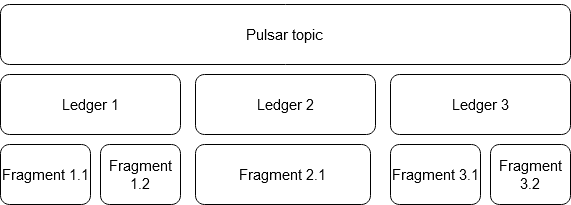
\includegraphics[width=6cm,height=2.5cm]{images/pulsar-topic.png}
	\caption{Underlying storage layers of a Pulsar topic.}
	\label{fig:pulsartopic}
\end{figure}
Although all these configuration options are from Bookkeeper which is used internally by Pulsar, Pulsar also allows users to configure them using its administrator tool to achieve the required level of fault tolerance in different use cases. When there are not enough Bookies to meet the configured ensemble size and quorum, writing request from clients will return an error. Moreover, whenever a Bookie node dies, fragment with records written on that node will not have enough Qw copies. In that case, if the auto recovery is enabled \cite{bookkeeperautoreco}, the Bookkeeper cluster can auto detect the failed node and replicate records on that Bookie to others to maintain Qw replicas for each record.  

\textbf{Flexible data retention policy}
As briefly mentioned in the general concept, a Pulsar topic can be read using Pulsar consumer. Whenever a consumer receives and processes successfully a message, it needs to send an acknowledgement back to the Pulsar broker. Based on that, Pulsar has two kinds of messages:
\begin{itemize}
	\item Able to delete: Messages which have been acknowledged by all consumers of the topic and messages on topic with no active consumers.
	\item Unable to delete: Messages which have not been acknowledge by all consumers of the topic.
\end{itemize}

\begin{figure}[h]
	\centering
	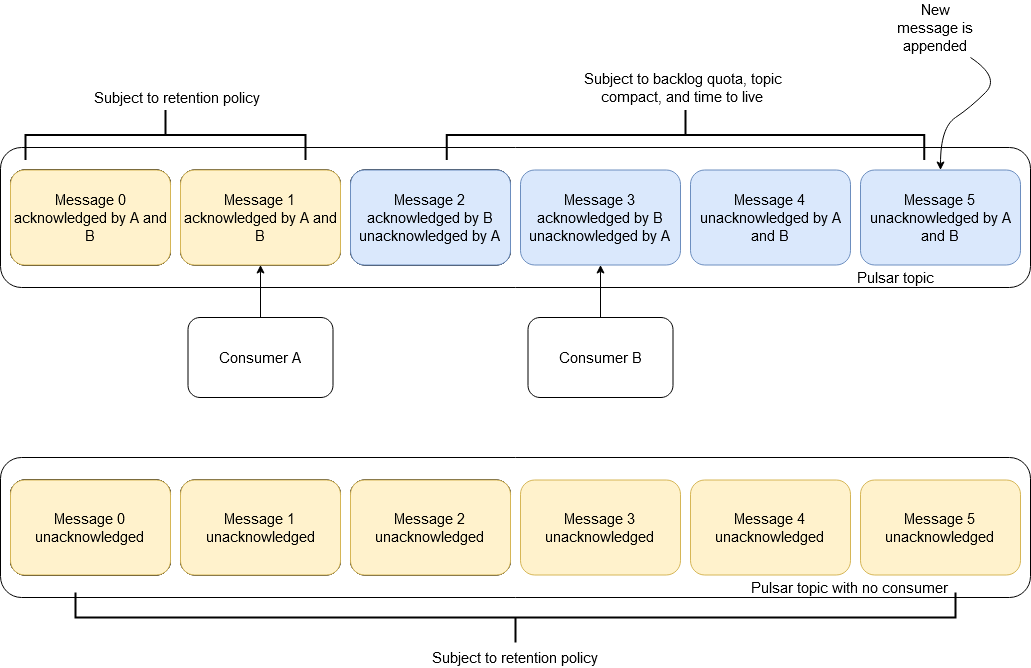
\includegraphics[width=12cm,height=7cm]{images/pulsar-retention.png}
	\caption{Message retention policy on Pulsar.}
	\label{fig:pulsarretention}
\end{figure}

By default, messages of the first type will be deleted the next time Pulsar does cleanup. Pulsar can be configured to retain these messages using retention policy \cite{pulsarretention}. User can set a time limit or a size limit for the retained messages on the topic. Whenever they exceed this limit, old messages will be deleted to keep the messages always within the limit. The size and time limits can be configured to be unlimited as well.

The second type of messages will always be retained by default. However, their size can grow too large. This can be controlled using backlog quota or time to live (TTL).

The backlog quota set a size limit on allowed unacknowledged messages of a topic. If this limit is exceeded, user can choose to reject new write request to topic or delete oldest unacknowledged messages. The main purpose of this configuration is not to save disk space. It aims at regulating the sending rate of producer in case slow consumers fall behind when consuming new messages by rejecting new sending request or reduce the number of unread messages.

On the other hand, TTL option focus on saving the disk space. It set a living time for unacknowledged messages. When the time expires, messages will be auto acknowledged to be subject to delete. 

Pulsar also provides the option for topic compaction \cite{pulsarcompact}. However, this is completely unrelated to saving disk space and in fact will increase the disk usage. In the compaction process, Pulsar will scan through the unacknowledged messages and make a new copy containing only latest message of each key value. Messages without key values will be overlooked by the compaction. This new compacted copy can be read by consumer when only latest values are relevant to speed up the processing.

These retention policies are only relevant to Pulsar consumer with its acknowledgement mechanism. In case of Pulsar reader, it does not acknowledge the consumption of messages to Pulsar and therefore does not determine which messages will be retained or deleted.

In summary, by default, messages on Pulsar will be deleted after being consumed by Pulsar consumer. However, it can be configured to retain messages as long as needed. Moreover, there is no option to selectively keep only latest messages to save disk space.

\large \textbf{NATS Streaming}\\
\normalsize
\textbf{Durable storage}

NATS streaming provides a pluggable persistence layer for durable storage of messages \cite{natsstorage}. However, by default, persistence storage is disabled and NATS streaming server only stores messages in-memory. NATS Streaming must be explicit configured to use durable storage. 

There are currently two storage options supported out-of-the-box which are file store and relational database store which are referred as SQL store in the NATS document. With file store, messages are stored in files on the disk of the server or in a network filesystem (NFS) mounted on the server. A directory is created for each channel in which messages of that channel are stored in log files. On the other hand, with SQL store, messages are persisted as records in an external relational database. All messages published to NATS Streaming are persisted in a messages table and each of them is uniquely identified by the ID number of the channel to which it belongs and an incremental sequence number. With these two provided storage options, once the producer of a message receive acknowledgement from the server, it is guaranteed that the message is durably persisted. Moreover, NATS Streaming also provides a storage interface which can be self-implemented by user to connect NATS to a different data store. 

\textbf{Event storage is fault tolerant}\\
NATS Streaming has two different clustering modes. In fault tolerance mode, all server instances are mounted to the same shared data store such as NFS or a shared database table depending on which persistence layer is used by the servers. NATS Streaming does not support data replication for fault tolerance of data with this mode. The shared data store can become the single point of failure. Once it goes down, data is not accessible or even worse lost. If fault tolerance of data is required, it relies entirely on users. For instance, users can implement data replication on the persistence layer themselves or use a fully managed storage service such as Amazon Elastic File System (EFS). 

Fault tolerance of event store is provided out-of-the-box by NATS Streaming with the clustering mode. In this mode, each node maintains a full copy of data in a separated data store. The nodes in NATS streaming cluster use Raft Consensus algorithm to replicate data \cite{raftalg}. Only the Raft leader node can take care of receiving requests for all channels and make copies on other nodes. Users only have to start up a NATS streaming cluster with a number of nodes and data will be auto replicated among them. Producers of message will receive acknowledgement once the replication process is finished. With Raft Consensus algorithm, a cluster with \emph{2n+1} node can tolerate up to \emph{n} node failures and continue to operate while guaranteeing no message loss. If there are more failures, the NATS Streaming cluster cannot accept new messages. It is recommended by NATS to limit the cluster size to only 3 or 5 nodes.

\begin{figure}[h]
	\centering
	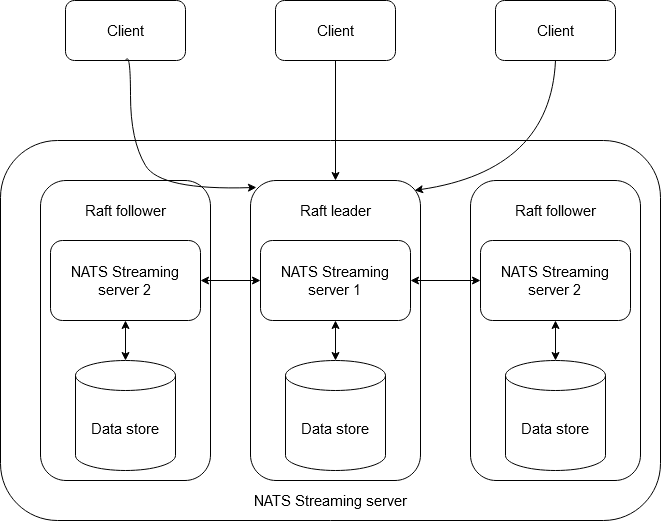
\includegraphics[width=12cm,height=7cm]{images/ft-eventstorage-nats.png}
	\caption{Fault tolerance of event storage on NATS Streaming in clustering mode.}
	\label{fig:natsftstorage}
\end{figure}

\textbf{Flexible data retention policy}\\
If persistence storage is enabled, all messages published to NATS Streaming will be retained whether they are consumed or not. User can specify the maximum number of channels, maximum size or number of messages of a channel, maximum retained time of each message \cite{natsstoragelimit}.

When the limits are exceeded, oldest messages will be deleted until the retained data falls below the maximum limitation. All of these policies can be set to unlimited to retain messages forever. However, there is no option to selectively retain messages on NATS Streaming server.







